
\newpage
\section{Motifs}

In this chapter we analyze the strucarl. The term motif referes
to... . Studies of \textcite{Song2005} and \textcite{Perin2011} show
stuff. Pernice2011, Sporns , Zhao2011.


\subsection*{Three-neuron patterns}

Here we investigate the occurrence of three-neuron patterns in the
anisotropic networks. \textcite{Song2005} reported a characteristic,
highly non-random motif distribution in rat's visual cortex (layer 5),
that was later confirmed by \textcite{Perin2011} in the rat's
somatosensory cortex (layer 5). 

There are 12 three-neuron motifs that represent connected simple
directed graphs, here labeled 4 to 16 to stay consistent with the
reports of Song et al. By analyzing connectivity in the different
sample graphs, three-neuron motif occurrences were recorded and
compared relative from Section~\ref{sec:two_neuron}

In anisotropic networks we found two-neuron pair probabilities of
occurrence of
\begin{align*} 
p_u & = 0.791336     &&\text{for unconnected pairs,}  \\
p_s & = 0.184151 &&\text{for single connections and}\\
p_r & = 0.024513  &&\text{for reciprocal connections.}
\end{align*}
Pattern 8, for example, has a probability of occurrence of 
\[
\mathbf{P}(X=8) = 6\, p_{u} p_{s} p_{r},
\]
where $X$ maps the motif the corresponding number as shown in . The
full probabilities are

\vspace{-0.9cm}
\begin{figure}[H]
  \begin{minipage}[c]{0.32\textwidth}
    \begin{align*}
      % \mathbf{P}(X=1) &    =   p_u^3  \\
      % \mathbf{P}(X=2) &    =   6 p_u p_u p_s\\
      % \mathbf{P}(X=3) &    =   3 p_u p_u p_r\\
      \mathbf{P}(X=4) &    =   3 p_s^2 p_u\\
      \mathbf{P}(X=5) &    =   3 p_s^2 p_u\\
      \mathbf{P}(X=6) &    =   6 p_s^2 p_u\\
      \mathbf{P}(X=7) &    =   6 p_s p_u p_r
    \end{align*}
  \end{minipage}%
  \begin{minipage}[c]{0.32\textwidth}
    \begin{align*}
      \mathbf{P}(X=\,\,\,9) &    =   3 p_r^2 p_u\\
      \mathbf{P}(X=10) &   =   6 p_s^3   \\
      \mathbf{P}(X=11) &   =   2 p_s^3    \\
      \mathbf{P}(X=12) &   =   3 p_s^2 p_r
    \end{align*}
  \end{minipage}%
  \begin{minipage}[c]{0.32\textwidth}
    \begin{align*}
      \mathbf{P}(X=13) &   =   6 p_s^2 p_r\\
      \mathbf{P}(X=14) &   =   3 p_s^2 p_r\\
      \mathbf{P}(X=15) &   =   6 p_s p_r^2\\
      \mathbf{P}(X=16) &   =   p_r^3.
    \end{align*}
  \end{minipage}
  \vspace{-0.9cm}
\end{figure}

Taking the probabilities of occurrence as computed from the two-neuron
connections as the expect, we identify overrepresentation. 

\begin{figure}[H]
  \centering
  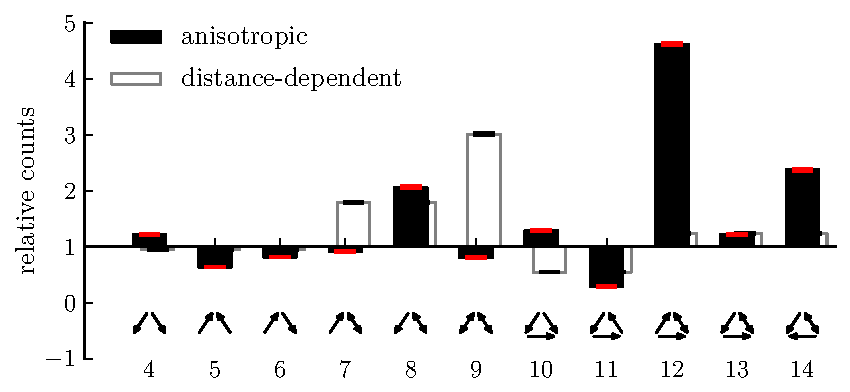
\includegraphics[width=0.95\linewidth]{%
    plots/4839ce41_aniso_dist.pdf}

    % \makebox{%
    % \hspace{1.23cm}\begin{overpic}[height=3.6cm]{%
    %     plots/15motifs.pdf}
    %   \put(32.3,44.9){\small 15}
    %   \put(40,42.9){
\includegraphics[width=0.5cm]{img/misc/song_motif_15.pdf}}
    % \end{overpic} 
    % \hspace{0.2cm}
    % \begin{overpic}[height=3.6cm]{%
    %     plots/16motifs.pdf}
    %   \put(54,83){\small 16}
    %   \put(68,79){
\includegraphics[width=0.5cm]{img/misc/song_motif_16.pdf}}
    % \end{overpic} 
    % }%

  \captionsetup{skip=8pt}
  \caption{\textbf{Relative occurrence of three-neuron patterns}
    Extracting the counts of three-node motifs in anisotropic (filled
    bars) and distance-dependent networks (unfilled bars), the
    quotient of the obtained count with the number of occurrences
    expected from the two-neuron connection probabilities in the
    networks (cf. Section~\ref{sec:two_neuron}) shows the over- and
    underrepresentation of specific motifs in the network (red and
    black errorbars are SEM). In anisotropic networks pattern 12, for
    example, appears around five times more often than we would expect
    from the occurrence two-neuron connections. The relative counts
    for anisotropic networks resemble the findings of
    \textcite{Song2005} and differ significantly from the counts in
    distance-dependent networks, implying that anisotropy has a strong
    influence on the relative occurrence of three-neuron
    patterns. (\smtcite{4839ce41}) }
  \label{fig:distance_3motif_compare}
\end{figure}


Interestingly, full do not appear (mean = ) in tuned anisotropic,
given evidence towards the incompleteness of the model.


To fully we ex. The results from give good evidence, however we find
that

\begin{figure}[H]
  \centering
  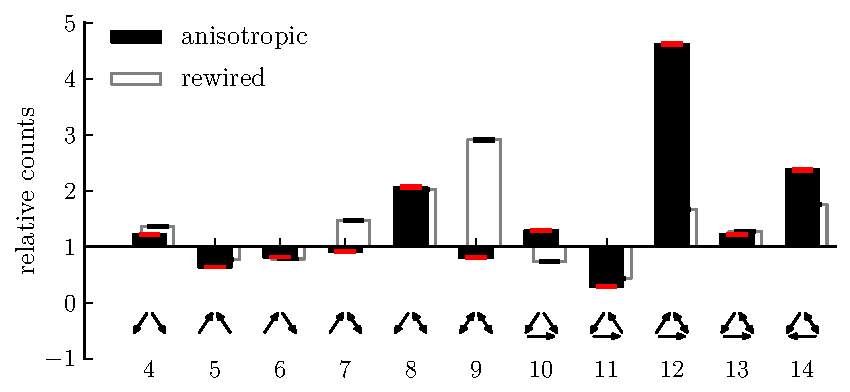
\includegraphics[width=0.95\linewidth]{%
    plots/4839ce41_aniso_rew.pdf}

  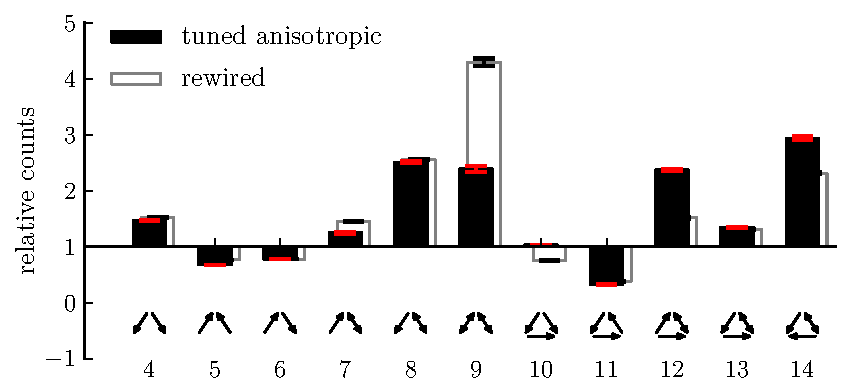
\includegraphics[width=0.95\linewidth]{%
    plots/4839ce41_tanfit_rew.pdf}

  \vspace{0.4cm}

  \makebox{%
    \hspace{1.208cm}%1.23
    \begin{overpic}[height=3.6cm]{%
        plots/4839ce41_motif15.pdf}
      \put(32.3,44.9){\small 15}
      \put(40,42.9){
\includegraphics[width=0.5cm]{img/misc/song_motif_15.pdf}}
    \end{overpic} 
    \hspace{0.19cm}
    \begin{overpic}[height=3.6cm]{%
        plots/4839ce41_motif16.pdf}
      \put(54,83){\small 16}
      \put(68,79){
\includegraphics[width=0.5cm]{img/misc/song_motif_16.pdf}}
    \end{overpic} 
  }%

  \captionsetup{skip=8pt}
  \caption{\textbf{Relative occurrence of three-neuron patterns}
    Extracting the counts of three-node motifs in anisotropic (filled
    bars) and distance-dependent networks (unfilled bars), the
    quotient of the obtained count with the number of occurrences
    expected from the two-neuron connection probabilities in the
    networks (cf. Section~\ref{sec:two_neuron}) shows the over- and
    underrepresentation of specific motifs in the network (red and
    black errorbars are SEM). In anisotropic networks pattern 12, for
    example, appears around five times more often than we would expect
    from the occurrence two-neuron connections. The relative counts
    for anisotropic networks resemble the findings of
    \textcite{Song2005} and differ significantly from the counts in
    distance-dependent networks, implying that anisotropy has a strong
    influence on the relative occurrence of three-neuron
    patterns. (\smtcite{4839ce41}) }
  \label{fig:distance_3motif_compare}
\end{figure}



Anisotropy in connectivity can for motifs 10, 12 and 14, however not
in motif 4. Additionally, anisotropy in connectivity causes for large
in motifs . Motif 9 is significantly underrepresented in anisotropic
networks, also reflecting the findings of Song et al.



\subsection*{Edge counts in neuron clusters}


% \begin{figure}[H]
%   \centering
%   \includegraphics[width=0.95\linewidth]{%
%     plots/7c826e10_test.pdf} 
%   \captionsetup{skip=8pt}
%   \caption{\textbf{Relative occurrence of three-neuron patterns}
%     Extracting the counts of three-node motifs in anisotropic (filled
%     bars) and distance-adependent networks (unfilled bars), the
%     quotient of the obtained count with the number of occurrences
%     expected from the two-neuron onnection probabilities in the
%     networks (rs =, ,, cfsdfg.) shows the over- and underrepresentation of
%     specific motifs in the network (red and black errorbars are
%     SEM). In anisotropic networks pattern number \enquote{12}, for
%     example, appears around five times more often than we would expect
%     from the occurrele the findings of
%     \textcite{Song2005} and differ significantly from the counts in
%     distance-dependent networks, implying that anisotropy has a strong
%     influence on the relative occurrence of three-neuron
%     patterns. (\smtcite{4839ce41}) }
%   \label{fig:distance_theory_compare}
% \end{figure}



% \begin{figure}[H]
%   \centering
%   \renewcommand{\tabcolsep}{0pt}
%   \setlength\extrarowheight{0pt}
%   \begin{tabular}{ll}
%     \begin{overpic}[width=0.5\textwidth]{%
%         /users/hoffmann/research/cn_k_test.pdf}
%       %\put(12,56){\small $\eta = 0$}
%     \end{overpic}
%     &
%     \begin{overpic}[width=0.5\textwidth]{%
%         /users/hoffmann/research/cn_k_test.pdf}
%       %\put(12,56){\small $\eta = 0.25$}
%     \end{overpic}
%     \\
%     \begin{overpic}[width=0.5\textwidth]{%
%         /users/hoffmann/research/cn_k_test.pdf}
%       %\put(12,56){\small $\eta = 0.5$}
%     \end{overpic}
%     &
%     \begin{overpic}[width=0.5\textwidth]{%
%         /users/hoffmann/research/cn_k_test.pdf}
%       % \put(12,56){\small $\eta = 0.75$}
%       %\put(4,-4){\small$0$}\put(78,-4){\small$200$}
%     \end{overpic}
%     \\
%     % \begin{overpic}[width=0.28\textwidth]{%
%     %     plots/77995b6b_in100.pdf}
%     %   \put(12,56){\small $\eta = 1$}
%     %   \put(4,-4){\small$0$}\put(78,-4){\small$200$}
%     % \end{overpic}
%     % & 
%     % \begin{overpic}[width=0.28\textwidth]{%
%     %     plots/77995b6b_indst.pdf}
%     %   \put(12,56){\small distance}
%     %   \put(4,-4){\small$0$}\put(78,-4){\small$200$}
%     % \end{overpic}
%     % \\
%   \end{tabular}
%   \caption{\textbf{In-degxree distrbution not affected by varying
%       degrees of anisotropy} 
%     (\smtcite{77995b6b}). }
%   \label{fig:in_degree_rewiring}
% \end{figure}



% \begin{figure}[htp]
%   \centering
 
%   \makebox{%
%     \hspace{1.23cm}
%     \begin{overpic}[height=3.6cm]{%
%         plots/4839ce41_motif15.pdf}
%       \put(32.3,44.9){\small 15}
%       \put(40,42.9){
\includegraphics[width=0.5cm]{img/misc/song_motif_15.pdf}}
%     \end{overpic} 
%     \hspace{0.19cm}
%     \begin{overpic}[height=3.6cm]{%
%         plots/4839ce41_motif16.pdf}
%       \put(54,83){\small 16}
%       \put(68,79){
\includegraphics[width=0.5cm]{img/misc/song_motif_16.pdf}}
%     \end{overpic} 
%   }%
%   \captionsetup{skip=7pt}
%   \caption{\textbf{Distance-independent overrepresentation of
%       reciprocal connections} Compaison of occurrences of one- and
%     bidirectionally connected neuron apairs in the tuned anisotropic
%     networks (gray) with profiles found by Perin et al.~(red), shows
%     that overrepresentation of bidirectional pairs is
%     distance-independent and not connected to anisotropy.  \textbf{A)}
%     Overall connection probability. (\smtcite{875505b0})}
%   \label{fig:perinadsf}
% \end{figure}


%%% Local Variables: 
%%% mode: latex
%%% TeX-master: "../dplths_document"
%%% End: 
